\documentclass[12pt]{article}

% =========================
% PACKAGES
% =========================
\usepackage[english]{babel}
\usepackage[utf8]{inputenc}
\usepackage[T1]{fontenc}
\usepackage{graphicx}
\usepackage{geometry}
\usepackage{setspace}
\usepackage{csquotes}
\usepackage{fancyhdr}
\usepackage{amsmath}
\usepackage{amssymb}
\usepackage{float}
\usepackage{caption}



% =========================
% BIBLIOGRAPHY
% =========================
\usepackage[
    backend=biber,
    style=numeric,
    sorting=nyt
]{biblatex}

\addbibresource{../references.bib}

% =========================
% PAGE SETUP
% =========================
\geometry{
    a4paper,
    margin=2.5cm,
    top=3.2cm
}
\setstretch{1.2}
\setlength{\headheight}{42pt}
\setlength{\headsep}{20pt}

% =========================
% Caption Setup
% =========================
\captionsetup[figure]{
    justification=centering,
    singlelinecheck=false,
    font=small,
    labelfont=bf
}

% =========================
% HEADER
% =========================
\pagestyle{fancy}
\fancyhf{}

\lhead{
\includegraphics[width=3.2cm]{../figures/banner_uandes.jpg}}
\rhead{
    \begin{tabular}{r}
        Lucas Zamora F. \\
        lzamora@miuandes.cl
    \end{tabular}
}

\renewcommand{\headrulewidth}{0.4pt}

% =========================
% HYPERLINKS
% =========================
\usepackage[
    colorlinks=true,
    linkcolor=blue,
    citecolor=blue,
    urlcolor=blue
]{hyperref}

\usepackage{bookmark}

% =========================
% DOCUMENT
% =========================
\begin{document}

% =========================
% COVER PAGE
% =========================
\begin{titlepage}
    \thispagestyle{empty}

    \begin{center}

        % =========================
        % TOP: VERSION
        % =========================
        \vspace*{0cm}
        {\small Version 0.1 --- Exploratory Draft}

        \vspace*{\fill}

        % =========================
        % CENTER BLOCK
        % =========================
        {\Large \textbf{Exploratory Research Document}}\\[0.8cm]

        {\Huge \textbf{Instance Space Analysis (ISA) and MATILDA}}\\[0.4cm]

        {\large Methodology, Pipeline and Output Interpretation}\\[0.6cm]

        {\large Part of the Master Thesis Research}\\[1.2cm]

        {\large Industrial Engineering}\\
        {\large School of Engineering and Applied Sciences}\\
        {\large Universidad de los Andes}

        \vspace*{\fill}

        % =========================
        % BOTTOM: AUTHOR + DATE
        % =========================
        {\Large Lucas Zamora F.}\\[0.3cm]

        {\large \today}

    \end{center}

\end{titlepage}

% =========================
% FRONT MATTER
% =========================
\tableofcontents
\newpage

\listoffigures
\newpage

\listoftables
\newpage

% =========================
% MAIN CONTENT
% =========================
\section{Introduction}

This document supports the exploratory stage of understanding Instance Space Analysis (ISA), MATILDA, and the interpretation of their outputs. Its purpose is to consolidate concepts, methodology, graphical interpretations, and implementation details relevant to the thesis work.

\section{Background: Instance Space Analysis (ISA)}

\subsection{Motivation and Limitations of Traditional Benchmarking}

Traditional approaches to algorithm benchmarking rely on evaluating performance over a fixed set of test instances and reporting aggregate statistics, such as average performance. However, this approach presents significant limitations. In particular, the conclusions drawn are highly dependent on the choice of test instances, which are often inherited from the literature without rigorous assessment of their diversity or representativeness.

As highlighted in \cite{smith-milesInstanceSpaceAnalysis2023}, two critical issues arise: (i) the lack of mechanisms to evaluate whether benchmark instances are sufficiently diverse and unbiased, and (ii) the inability to understand how algorithm performance varies with respect to instance characteristics. As a result, important insights regarding algorithm strengths and weaknesses remain hidden when relying solely on aggregated performance metrics.

Instance Space Analysis (ISA) addresses these limitations by providing a framework that explicitly models the relationship between instance characteristics and algorithm performance.

\subsection{Conceptual Framework}

The ISA methodology extends the classical Algorithm Selection Problem introduced by Rice in \cite{AlgorithmSelectionProblem1976}, where the goal is to select the best-performing algorithm for a given problem instance based on its features.

Formally, ISA considers six fundamental components:

\begin{itemize}
    \item A problem space $\mathcal{P}$, representing all possible instances of a problem domain.
    \item A subset of instances $\mathcal{I} \subset \mathcal{P}$ for which empirical data is available.
    \item A feature space $\mathcal{F}$, where each instance $x \in \mathcal{I}$ is represented by a feature vector $\mathbf{f}_x \in \mathbb{R}^m$.
    \item An algorithm space $\mathcal{A}$, containing the set of candidate algorithms.
    \item A performance space $\mathcal{Y}$, where each value $y_{\alpha,x}$ measures the performance of algorithm $\alpha \in \mathcal{A}$ on instance $x$.
    \item A meta-data set consisting of the matrices
    \[
    \mathbf{F} \in \mathbb{R}^{m \times n}, \qquad \mathbf{Y} \in \mathbb{R}^{a \times n},
    \]
    where $n$ is the number of instances and $a$ is the number of algorithms.
\end{itemize}

Within the classical framework, this meta-data is used to learn a selection mapping that predicts the best algorithm for a given instance. ISA extends this paradigm by introducing a new objective: the construction of a low-dimensional representation of the instance space that enables visualization and interpretation of algorithm behavior.

\vspace*{1cm}

\begin{figure}[H]
    \centering
    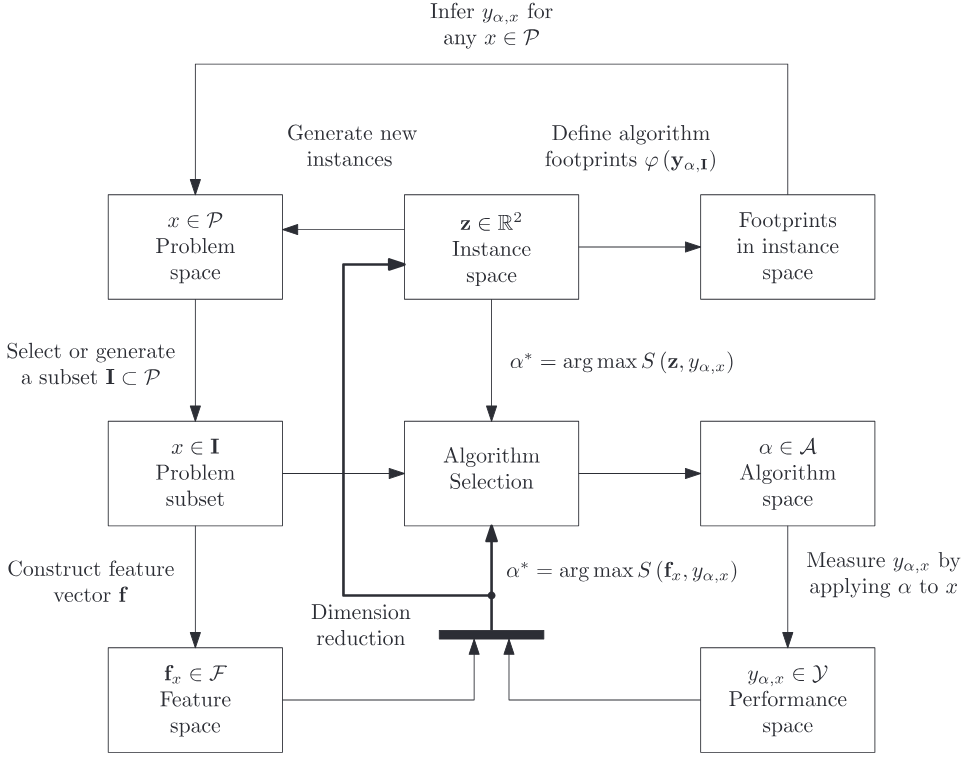
\includegraphics[width=0.9\textwidth]{../figures/isa_framework.png}
    \caption{Summary of the Instance Space Analysis (ISA) framework, reproduced from \cite{smith-milesInstanceSpaceAnalysis2023}.}
    \label{fig:isa_framework}
\end{figure}

\newpage
\subsection{Interpretation of the ISA Framework}

Figure~\ref{fig:isa_framework} presents a conceptual overview of the Instance Space Analysis (ISA) framework. The diagram illustrates how problem instances, their features, and algorithm performance are interconnected within a unified analytical structure.

The process begins with the \textit{problem space} $\mathcal{P}$, which represents the universe of all possible problem instances. From this space, a subset $\mathcal{I} \subset \mathcal{P}$ is selected or generated for empirical analysis. Each instance $x \in \mathcal{I}$ is then characterized by a feature vector $\mathbf{f}_x \in \mathcal{F}$, defining its position in the feature space.

A key step in ISA is the transformation of the feature space into a low-dimensional instance space, enabling visualization and supporting the interpretation of algorithm behavior.

Within the instance space, algorithm performance is analyzed through the concept of \textit{algorithm selection}. Given a point $\mathbf{z}$, the framework aims to identify the algorithm $\alpha^* \in \mathcal{A}$ that maximizes a performance measure $S(\cdot)$, effectively linking instance characteristics with expected algorithm behavior.

The \textit{performance space} $\mathcal{Y}$ captures the empirical results obtained by applying each algorithm $\alpha \in \mathcal{A}$ to instances $x \in \mathcal{I}$. These measurements provide the foundation for evaluating and comparing algorithm performance across different regions of the instance space.

An important extension introduced by ISA is the notion of \textit{algorithm footprints}, which represent regions of the instance space where a given algorithm performs well. These footprints allow for a geometric interpretation of algorithm strengths and weaknesses, enabling a deeper understanding of performance variability.

Finally, the framework highlights an iterative feedback loop. Insights obtained from the instance space can be used to generate new problem instances, refine feature definitions, or improve algorithm selection strategies. This iterative process is fundamental to constructing a representative and informative instance space.

\subsection{Instance Space Representation}

A central contribution of ISA is the projection of instances from the high-dimensional feature space $\mathcal{F}$ into a two-dimensional instance space. Each instance $x$ is mapped to a point $\mathbf{z} \in \mathbb{R}^2$, such that geometric relationships reflect similarities in instance characteristics and algorithm performance.

This projection is constructed to preserve meaningful structure, enabling the identification of regions associated with different levels of difficulty for algorithms. As a result, the instance space provides a visual and analytical tool to explore how algorithm performance varies across different types of instances.

\subsection{Algorithm Footprints}

Within the instance space, ISA introduces the concept of \textit{algorithm footprints}, defined as regions where an algorithm is expected to perform well based on empirical evidence.

A footprint is characterized by several properties:

\begin{itemize}
    \item \textbf{Location}: indicates the types of instances where the algorithm performs well.
    \item \textbf{Area}: reflects the robustness of the algorithm across the instance space.
    \item \textbf{Density}: measures the strength of supporting empirical evidence.
    \item \textbf{Purity}: quantifies the consistency of performance within the region.
\end{itemize}

This representation allows for a more nuanced comparison between algorithms, revealing complementary strengths and weaknesses that are not observable through average performance metrics.

\subsection{Insights Enabled by ISA}

By combining feature information, performance data, and geometric representation, ISA enables:

\begin{itemize}
    \item Identification of regions where specific algorithms dominate.
    \item Detection of biases or gaps in benchmark instance sets.
    \item Understanding of how instance characteristics influence algorithm performance.
    \item Support for automated algorithm selection through learned mappings.
\end{itemize}

Furthermore, ISA is inherently iterative: the analysis of the instance space may reveal the need for additional instances, features, or algorithms, leading to progressively more informative representations.



% =========================
% BIBLIOGRAPHY
% =========================
\newpage
\printbibliography

\end{document}